\newpage
\appendix
\section{Appendices}


\subsection{Models}
\label{appendix:models}

\subsubsection{SimCLR}
SimCLR model \cite{simclrref} is a self-supervised learning method that aims to learn representations of the input data by comparing different augmented versions of the same input via contrastive loss in the latent space. The authors used the combination of random crop and colour distortion as augmentation methods. Pre-trained ResNet-18 \cite{resnetref} or Densenet-121 \cite{densenet} was used as an encoder on top of which a projection head with two linear layers and ReLU activation function was trained for 100 epochs. Hyperparameters used for training are in the table \ref{table:SimCLR hyperparemeters}.

\begin{table}[H]
    \centering
    \begin{tabular}{ll}
    \hline
                    Name & Value   \\
    \hline
     Optimizer & SGD\\
     Learning rate & 0.6\\
     Momentum   & 0.9\\
     Weight decay & $1\times10^{-6}$\\
     Temperature & 0.5\\
    \hline
    \end{tabular}
\caption{SimCLR hyperparameters.}
\label{table:SimCLR hyperparemeters}
\end{table}

\subsubsection{ECG5000 autoencoder}
We used the Recurrent Autoencoder that the authors used which consists of an encoder with an embedding dimension of 64, two LSTM layers and a decoder with two LSTMs and a final Linear layer. The model was trained to minimize the reconstruction loss given by \begin{math}L_{rec}(x)=\sum_{t=1}^{T}\left | x_{t}-\left [ \mathbf{f_{d}} \circ \mathbf{f_{e}(x)}\right ]_{t} \right | \end{math}, where $\mathbf{x}$ is a vector representing one time series sample, $T$ is the resolution of the heartbeat ($T=140$) and $\mathbf{f_{e}}$ and $\mathbf{f_{d}}$ stand for the encoder and decoder functions. The model was trained for 150 epochs using the Adam optimizer.
\\

% MNIST autoencoder for pretext - Mara
\subsubsection{MNIST autoencoder - Pretext Tasks} 
For each pretext task, a new autoencoder is trained. Each autoencoder is trained for 100 epochs, using the Adam optimizer, patience 10, and the same hyperparameters as presented in the paper. The classifier used follows the same architecture as the encoder used for the autoencoder, with an additional Softmax layer producing class probabilities. The pretext tasks tested are denoising, reconstruction, and inpainting, and for each pretext task the objective is to minimize their denoising, reconstruction, and inpainting loss accordingly as shown in equations \ref{eq:autoencoder_denoising}, \ref{eq:autoencoder_reconstruction}, \ref{eq:autoencoder_inpainting}. More details about these equations can be found in the original paper in Appendix C.1 and Appendix C.2.
\\

\begin{equation}\label{eq:autoencoder_denoising}
    L_{den}(x)=\mathop{\mathbb{E}_{\varepsilon}} [\mathbf{x} - \mathbf{f_{d}} \circ \mathbf{f_{e}(x + \varepsilon)} ] ^ {2}
\end{equation}

\begin{equation}\label{eq:autoencoder_reconstruction}
    L_{rec}(x)=[\mathbf{x} - \mathbf{f_{d}} \circ \mathbf{f_{e}(x)} ] ^ {2}
\end{equation}

\begin{equation}\label{eq:autoencoder_inpainting}
    L_{in}(x)=\mathop{\mathbb{E}_{M}} [\mathbf{x} - \mathbf{f_{d}} \circ \mathbf{f_{e}(M \odot x)} ] ^ {2}
\end{equation}

% Dsprites- d-VAE Andreas
\subsubsection{Disentangled Variational Autoencoder (VAE)}
We used the provided code for VAE experiments and we ran two versions of disentangled VAEs: $\beta$-VAE \citep{betavae} and TC-VAE \citep{tcvae}, with beta values $\beta$ $\in$ \{1, 5, 10\}. We trained the models for 100 epochs on MNIST and dSprites datasets (90\%-10\% train-test split) using $d_H$ = 3 and $d_H$ = 6 latent units respectively. We ran 5 times for every disentangled VAE type for each $\beta$. Thus, in total, 30 models were trained.


\subsection{Datasets}
\label{appendix:datasets}
\subsubsection{MNIST} This is a black-and-white image dataset containing digits from 0 to 9. Each image is 28x28 pixels. For the feature importance experiment the denoising autoencoder was trained on the entire training set and the attribution methods were tested on the whole training set. The example importance experiments were run on a subset of 1000 training and 1000 testing samples. 

\subsubsection{Fashion MNIST} It is similar to MNIST, but instead of digits, the images depict clothing items that belong to 10 different categories. The partitioning was done in the same way as for MNIST.

\subsubsection{CIFAR-10} This RGB image dataset contains 32x32 pixel pictures of objects corresponding to 10 categories. A 50000/10000 partition was used for the feature importance experiment, while for determining the most important examples, they used a subset of 1000/1000.

\subsubsection{ECG5000} Is a time series dataset that describes the heartbeat of a patient. Each time series describes one single heartbeat with a resolution of 140 time steps. This dataset was split into 4000 training and 1000 testing samples when conducting the experiments.

\subsubsection{dSprites} This is a synthetic dataset of images showing 2D shapes generated from the following latent factors: colour, shape, scale, rotation, x and y positions of a sprite. The dataset has a total of 737280 images, from which 10\% were used at test time. 

\newpage
\subsection{Reproducing Pretext Experiments}
\label{appendix:pretext_visualisations}

\subsubsection{Visualisations}

We visualise the top examples produced by different pretext tasks as well as their saliency maps for qualitatively interpreting the results. The results are shown in Figure \ref{fig:topex_pretext} and Figure \ref{fig:saliency_maps_pretext}.

\begin{figure}[H]
    \centering
    \includegraphics[width=14cm]{images/top_pretext.png}
    \caption{Label-free top example for various pretext tasks.}
    \label{fig:topex_pretext}
\end{figure}

\begin{figure}[H]
    \centering
    \includegraphics[width=14cm]{images/saliency_pretext.png}
    \caption{Label-free saliency for various pretext tasks.}
    \label{fig:saliency_maps_pretext}
\end{figure}

\subsubsection{ROAR Test}

The original paper also computes an additional test supporting the label-free feature importance method. The test follows the same consistency check for feature importance, with a difference in first removing the most important pixels, and then training the autoencoder on the modified data. We compare results with the original paper in Figure \ref{fig:roar_test_result} and obtain a similar trend.

\begin{figure}[H]
     \centering
     \begin{subfigure}[b]{0.45\textwidth}
         \centering
         \includegraphics[width=\textwidth]{images/roar_us.png}
         \caption{Our result.}
         \label{fig:mnist}
     \end{subfigure}
     \hfill
     \begin{subfigure}[b]{0.45\textwidth}
         \centering
         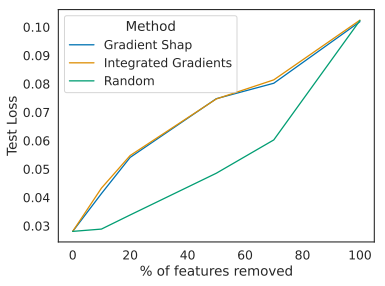
\includegraphics[width=\textwidth]{images/roar_them.png}
         \caption{Their result.}
         \label{fig:ecg}
     \end{subfigure}
     \hfill
    \caption{Comparing ROAR test results.}
    \label{fig:roar_test_result}
\end{figure}

\subsection{Experiments on Fashion MNIST}
\label{appendix:pretext_visualisations_fmnist}

\subsubsection{Example consistency}
%It can be seen in Figure \ref{fig:ex-feat-importance-fashion} that the same trends as for the other datasets hold for Fashion MNIST: the representation shift increases abruptly when we perturb the most important pixels, meaning that we managed to identify the key features for the encoder to come up with a representation and also the similarity rate between the most important examples is much higher than for the least important ones, showing that the method allows the identification of training samples related to test examples in the label-free setting.
% \begin{figure}[H]
%      \begin{subfigure}[b]{0.5\textwidth}
%          \centering
%          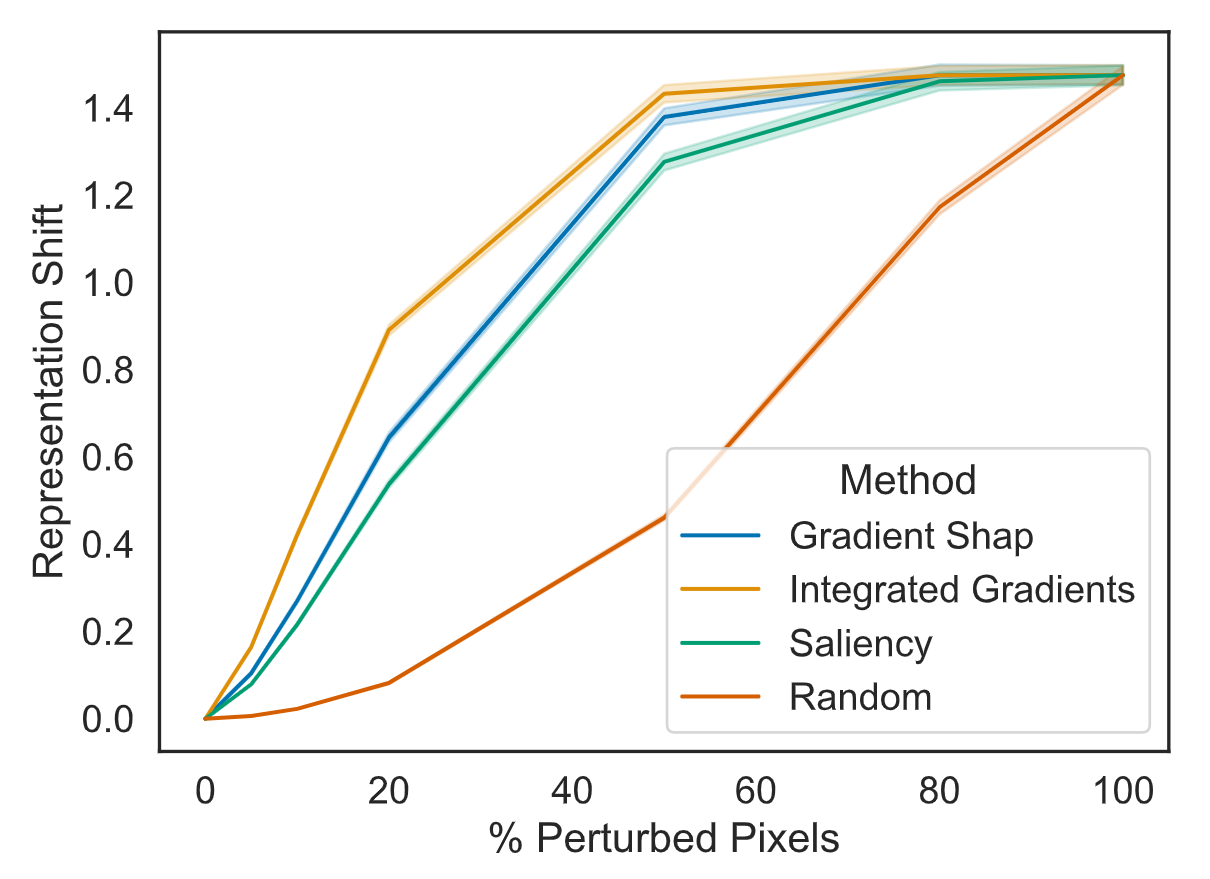
\includegraphics[width=\textwidth]{images/feature_consistency_fmnist.png}
%          \caption{Feature importance}
%          \label{fig:ecg}
%      \end{subfigure}
%      \hfill
%      \begin{subfigure}[b]{0.5\textwidth}
%          \centering
%          \includegraphics[width=\textwidth]{images/example_consistency_fmnist.png}
%          \caption{Example importance}
%          \label{fig:cifar}
%      \end{subfigure}
%         \caption{Consistency check for label-free feature and example importance on Fashion MNIST.}
%         \label{fig:ex-feat-importance-fashion}
% \end{figure}
It can be seen in Figure \ref{fig:fashion_example} that the same trend as for the other datasets holds for Fashion MNIST when testing the example consistency: the similarity rate between the most important examples is much higher than for the least important ones, showing that the method allows the identification of training samples related to test examples in the label-free setting.
\begin{figure}[H]
    \centering
    \includegraphics[width=10cm]{images/example_consistency_fmnist.png}
    \caption{ Consistency check for label-free example importance on Fashion MNIST. }
    \label{fig:fashion_example}
\end{figure}


\subsubsection{Quantitative analysis for pretext tasks}
Table \ref{table:pc_saliency_fmnist} and Table \ref{table:pc_example_fmnist} show the Pearson correlation coefficients of representations learned for different pretext tasks on Fashion MNIST dataset. The Pearson scores range from .31 to .49 corresponding to moderate positive correlation for saliency maps and from .07 to .31 corresponding to weak correlations for example importance.

\begin{table}[H]
    \centering
    \begin{tabular}{lllll}
    \hline
                    PEARSON & RECON. & DENOIS. & INPAINT. & CLASSIF.   \\
    \hline
     \multicolumn{1}{l|}{RECON.}     &  &  &  &   \\
     \multicolumn{1}{l|}{DENOIS.}     & $.49 \pm .05$  & &  &   \\
     \multicolumn{1}{l|}{INPAINT.}   & $.43 \pm .02$  & $.45 \pm .02$ &  &  \\
     \multicolumn{1}{l|}{CLASSIF.}   & $.37 \pm .01$  & $.36 \pm .02$  & $.31 \pm .03$ &    \\
    \hline
    \end{tabular}
\caption{Pearson correlation for saliency maps (avg +/- std).}
\label{table:pc_saliency_fmnist}
\end{table}

\begin{table}[H]
    \centering

    \begin{tabular}{lllll}
    \hline
                    PEARSON & RECON. & DENOIS. & INPAINT.  & CLASSIF.  \\
    \hline
     \multicolumn{1}{l|}{RECON.}     &  &  &  &  \\
     \multicolumn{1}{l|}{DENOIS.}    & $.27 \pm .06$  &  &  &   \\
     \multicolumn{1}{l|}{INPAINT.}   & $.30 \pm .03$  & $.31 \pm .09$ &  &  \\
     \multicolumn{1}{l|}{CLASSIF.}   & $.07 \pm .02$  & $.07 \pm .03$ & $.07 \pm .03$ &  \\
    \hline
    \end{tabular}
    
\caption{Pearson correlation for example importance (avg +/- std).}
\label{table:pc_example_fmnist}
\end{table}

\subsubsection{Qualitative analysis for pretext tasks}
The most important examples can be seen in Figure \ref{fig:topex_pretext_fmnist} and the saliency maps can be visualized in Figure \ref{fig:saliency_maps_pretext_fmnist}. By plotting these images we can better understand the choice of most important examples: if we look at the saliency maps for the sneaker image, we see that only the inpainting and the classification representations focus on the midsole and outsole of the shoe, leading to having more relevant top examples to the test image for these tasks.

\begin{figure}[H]
    \centering
    \includegraphics[width=14cm]{images/top_examples_fmnist.png}
    \caption{Top examples for sandal, shirt, sneaker, bag and ankle boot categories.}
    \label{fig:topex_pretext_fmnist}
\end{figure}

\begin{figure}[H]
    \centering
    \includegraphics[width=13cm]{images/saliency_fmnist.png}
    \caption{Saliency maps.}
    \label{fig:saliency_maps_pretext_fmnist}
\end{figure}

\subsection{CIFAR-10 masked images}
% \begin{figure}[H]
%     \centering
%     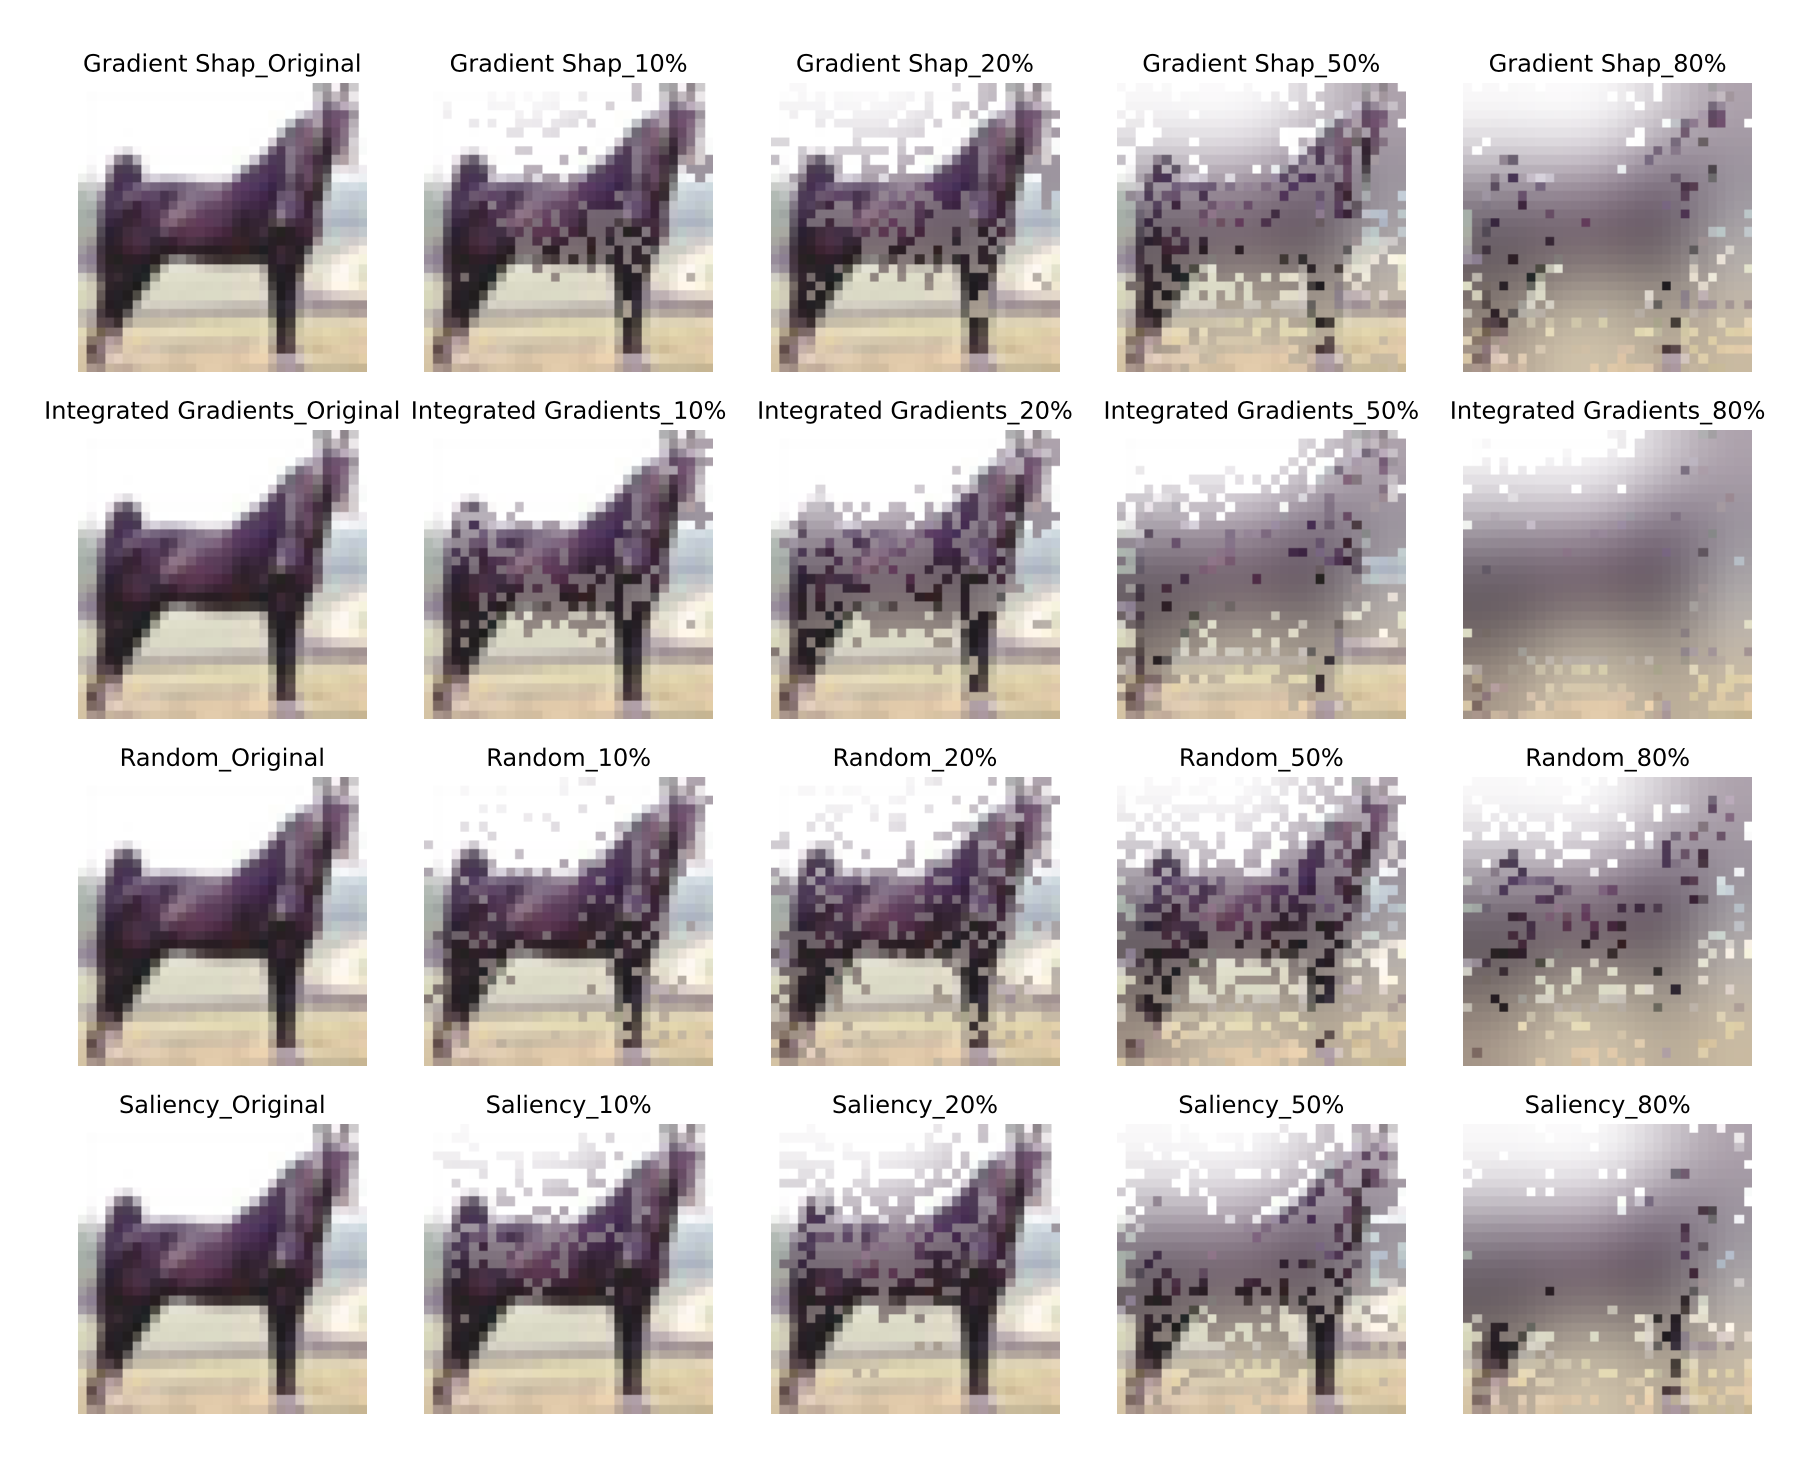
\includegraphics[width=12cm]{images/blurred horse.png}
%     \caption{Example of masked image from CIFAR-10 dataset for blurred mask}
%     \label{fig:blurred_horse}
% \end{figure}


\begin{figure}[H]
    \centering
    \includegraphics[width=12cm]{images/black horse.png}
    \caption{Example of masked image from CIFAR-10 dataset for black pixel mask}
    \label{fig:black_horse}
\end{figure}

\subsection{Explainability analysis with different attribution methods}
\label{appendix:explainability_attr_methods}

\subsubsection{Integrated Gradients}

For the \textit{pretext experiment}, we analyse the results \textbf{quantitatively} in Table \ref{table:pretext_integrated_grads_features} and Table \ref{table:pretext_integrated_grads_examples} and \textbf{qualitatively} in Figure \ref{fig:saliency_maps_pretext_integrated_grads} and Figure \ref{fig:topex_pretext_integrated_grads}. Moreover, for the \textit{VAE experiment}, we analyse the results \textbf{quantitatively} in Figure \ref{fig:vae_integrated_grads_quantitative} and \textbf{qualitatively} in Figure \ref{fig:vae_integrated_grads_qualitative}. Both experiments use label-free Integrated Gradients as their attribution method.

\begin{table}[H]
    \centering
    \begin{tabular}{lllll}
    \hline
                   PEARSON & RECON.   & DENOIS.       & INPAINT.      & CLASSIF.   \\
    \hline
     RECON. &  &  &  &  \\
     DENOIS.      & $0.45 \pm 0.06$  &  &  &    \\
     INPAINT.     & $0.43 \pm 0.08$  & $0.45 \pm 0.05$ &    &   \\
     CLASSIF. & $0.39 \pm 0.03$  & $0.4 \pm 0.02$  & $0.35 \pm 0.05$ &    \\
    \hline
    \end{tabular}
\caption{Pearson correlation for saliency maps (avg +/- std) using label-free Integrated Gradients.}
\label{table:pretext_integrated_grads_features}
\end{table}

\begin{table}[H]
    \centering
    \begin{tabular}{lllll}
\hline
               PEARSON & RECON.   & DENOIS.       & INPAINT.      & CLASSIF.   \\
\hline
 RECON. &    & &  &   \\
 DENOIS.      & $0.14 \pm 0.04$  &    &  &   \\
 INPAINT.     & $0.18 \pm 0.04$  & $0.21 \pm 0.04$ &    &    \\
 CLASSIF. & $0.09 \pm 0.02$  & $0.09 \pm 0.02$ & $0.1 \pm 0.01$  &     \\
\hline
\end{tabular}
\caption{Pearson correlation for example importance (avg +/- std) using label-free Integrated Gradients.}
\label{table:pretext_integrated_grads_examples}
\end{table}

\begin{figure}[H]
    \centering
    \includegraphics[width=10cm]{images/vae_integrated_grads.png}
    \caption{Pearson correlation between saliency maps for different values of \(\beta\) using label-free Integrated Gradients.}
    \label{fig:vae_integrated_grads_quantitative}
\end{figure}

\begin{figure}[H]
    \centering
    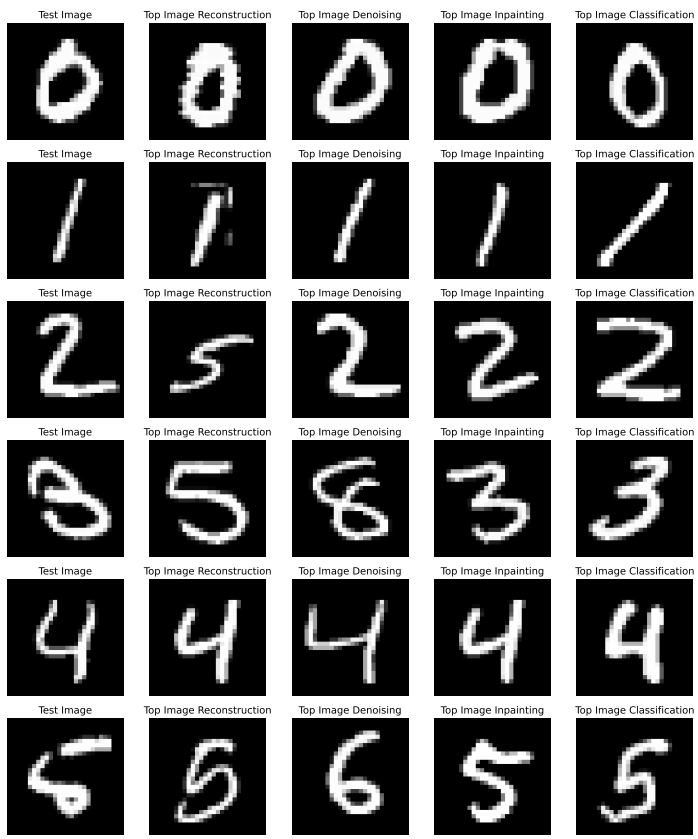
\includegraphics[width=12cm]{images/pretext_top_integrated_grads.png}
    \caption{Top examples using label-free Integrated Gradients.}
    \label{fig:topex_pretext_integrated_grads}
\end{figure}

\begin{figure}[H]
    \centering
    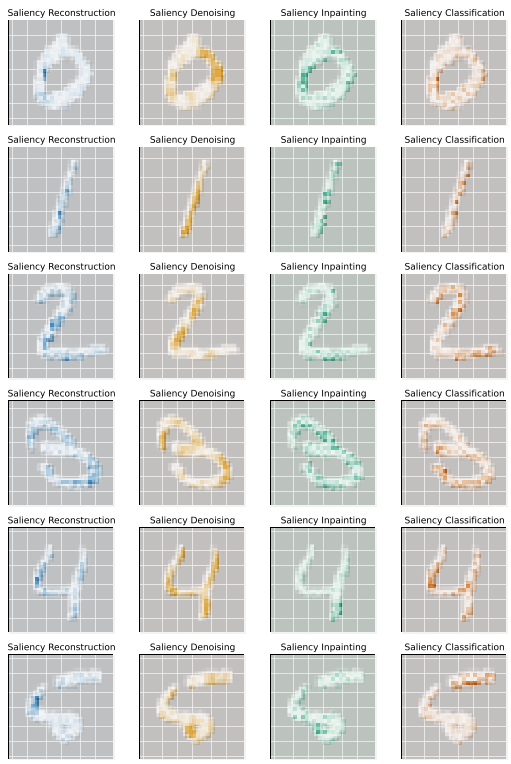
\includegraphics[width=12cm]{images/pretext_saliency_integrated_grads.png}
    \caption{Saliency maps using label-free Integrated Gradients.}
    \label{fig:saliency_maps_pretext_integrated_grads}
\end{figure}

\begin{figure}[H]
    \centering
    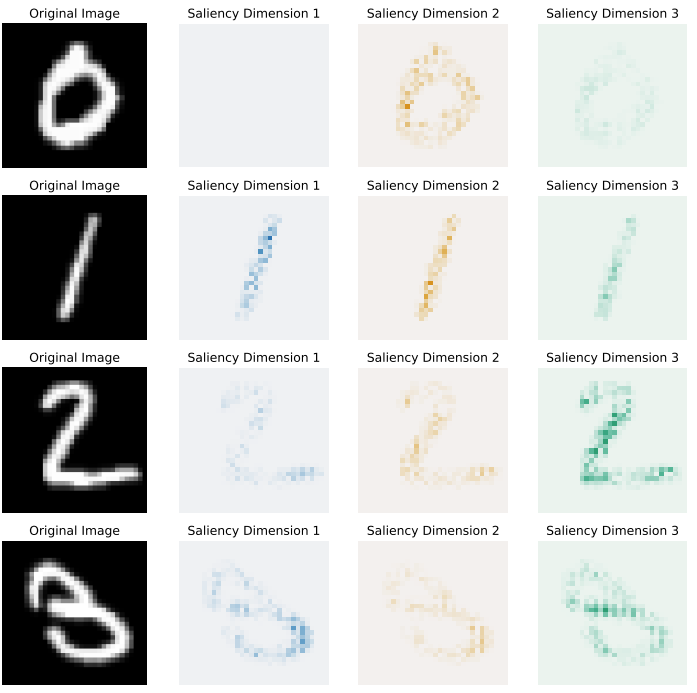
\includegraphics[width=12cm]{images/vae_integrated_grads_qualiative.png}
    \caption{Saliency maps for each unit of the disentangled VAEs using Integrated Gradients.}
    \label{fig:vae_integrated_grads_qualitative}
\end{figure}

% \subsubsection{Saliency}

% For the \textit{pretext experiment}, we analyse the results \textbf{quantitatively} in Table \ref{} and \textbf{qualitatively} in Figure \ref{}. Moreover, for the \textit{VAE experiment}, we analyse the results \textbf{quantitatively} in Table \ref{} and \textbf{qualitatively} in Figure \ref{}. Both experiments use label-free Saliency as their attribution method.
\subsection{DenseNet Experiments}
 \begin{figure}[H]
    %\centering
    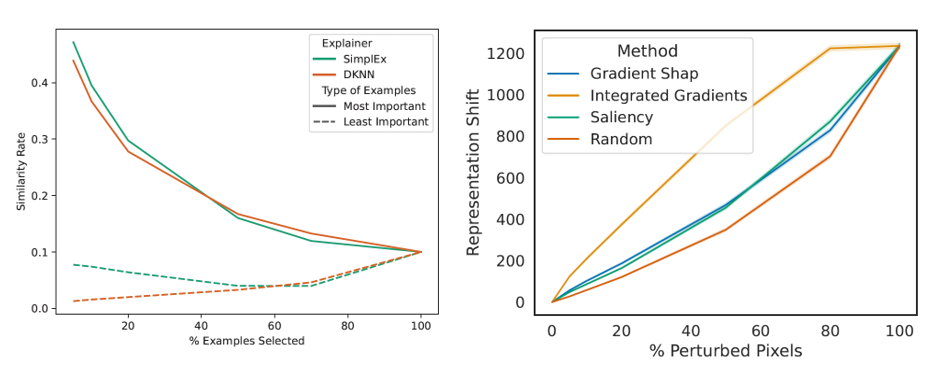
\includegraphics[width=13cm]{images/cifar_densenet.png}
    \caption{ Consistency check for label-free example importance (left) and label-free feature importance (right) using DenseNet121 on CIFAR-10 dataset. }
    \label{fig:cifar_densenet}
\end{figure}

